\documentclass[dvisvgm,tikz]{standalone}
\begin{document}
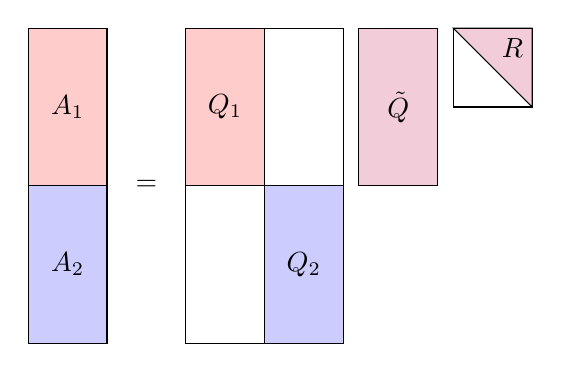
\begin{tikzpicture}

\filldraw[fill=red!20] (0,2) rectangle (1,4);
\filldraw[fill=blue!20] (0,0) rectangle (1,2);
\node at (0.5,3) {$A_1$};
\node at (0.5,1) {$A_2$};
\draw (2,0) rectangle (4,4);
\filldraw[fill=red!20] (2,2) rectangle (3,4);
\filldraw[fill=blue!20] (3,0) rectangle (4,2);
\node at (2.5,3) {$Q_1$};
\node at (3.5,1) {$Q_2$};

\draw (6.4,3) rectangle (5.4,4);
\filldraw[fill=purple!20] (4.2,4) rectangle (5.2,2);
\filldraw[fill=purple!20] (5.4,4) -- (6.4,3) -- (6.4,4) -- cycle;
\node at (4.7,3) {$\tilde{Q}$};
\node at (6.15,3.75) {$R$};

\node at (1.5,2) {$=$};

\end{tikzpicture}
\end{document}
